\section{Introduction}

Large language models (LLMs) such as GPT-4~\citep{openai2023gpt}, Claude~\citep{bai2022training}, and Llama~\citep{touvron2023llama,touvron2023llama2} are rapidly reinventing today's applications. 
Many companies are racing to deploy LLMs in their vertical domains, such as search, chatbots, and virtual assistants. Since most of these applications demand low latency, optimizing LLM serving latency is of vital importance and can directly translate into better quality of service and cost reduction.

The latency of today's LLM service is unfortunately very high. This is primarily because serving a user query requires multiple serial evaluations of the LLM, each generating only one token of the response.
An emerging solution to reduce the latency is speculative decoding. Speculative decoding employs a smaller model to speculate multiple output tokens of the target (large) model, then lets the target LLM verify these speculations in parallel. Then, if the verification of a token fails, the large model must recompute from that point. Therefore, the performance of speculative decoding primarily depends on the speculation accuracy of the small model. In the presence of diverse text inputs, %
the accuracy of existing speculative decoding methods is unfortunately not very high, due to the capability gap between the draft and target model. Employing a larger, more accurate model however defeats the purpose of speculative decoding as it potentially increases latency.

To address this challenge, we introduce a novel method, \emph{online speculative decoding}, specifically designed for online LLM services.
The method leverages the abundant redundant compute, termed as ``spare flops,'' available in a typical LLM serving cluster to continuously retrain (multiple) small draft models through online learning on query data posted to the LLM service. Our approach is simple and offers several significant advantages.
First, user queries to a specific LLM service often exhibit a common domain-specific distribution~\citep{zheng2023lmsys}, reflecting shared usage patterns.
While accurately speculating the larger model's outputs on \emph{any diverse input} is challenging, it is feasible to enhance the draft model's prediction accuracy, \emph{only for similar inputs posted to the service}, characterized by the query distribution. This can be achieved by finetuning the draft model on user query distribution or finetuning multiple draft models, each on a cluster of the query distribution, and selecting the appropriately specialized draft model to speculate based on the class of inputs they are trained on. As shown in~\S\ref{sec:eval:online_evaluation}, we show that it is possible to train multiple draft models, each for a different language or topic. 
Second, the primary bottleneck for transformer-based LLM inference is the accelerator's memory bandwidth, as generating each word requires loading the model weights from HBM to SRAM as well as reading the KV cache on all previous words. 
This results in a substantial amount of unused compute, especially during non-spike traffic hours~\citep{spector2023accelerating,chen2023accelerating,kwon2023efficient}, in an LLM serving cluster. We demonstrate that these spare FLOPs can be effectively repurposed for online retraining of draft models, with inconspicuous retraining cost (\S\ref{sec:analysis}).
Third, since tuning is performed online, the draft models continuously evolve over time based on the observed query data, which ensures high speculation accuracy even when faced with shifts in query distribution.






Based on these insights, we develop an online speculative decoding framework to improve the efficiency of online LLM serving. 
To align the draft model with the target model on a newly observed user query, we develop a new online learning algorithm based on Generalized Knowledge Distillation (GKD)~\citep{gu2023knowledge,agarwal2023gkd}. The algorithm keeps track of the recent queries that the draft model has speculated incorrectly, and forces the draft model to emulate the target model's outputs on these queries. The algorithm performs GKD-based gradient update opportunistically only when spare flops are available, hiding the overhead. 

\begin{figure}[h]       
    \centering
    \label{fig:arch}
    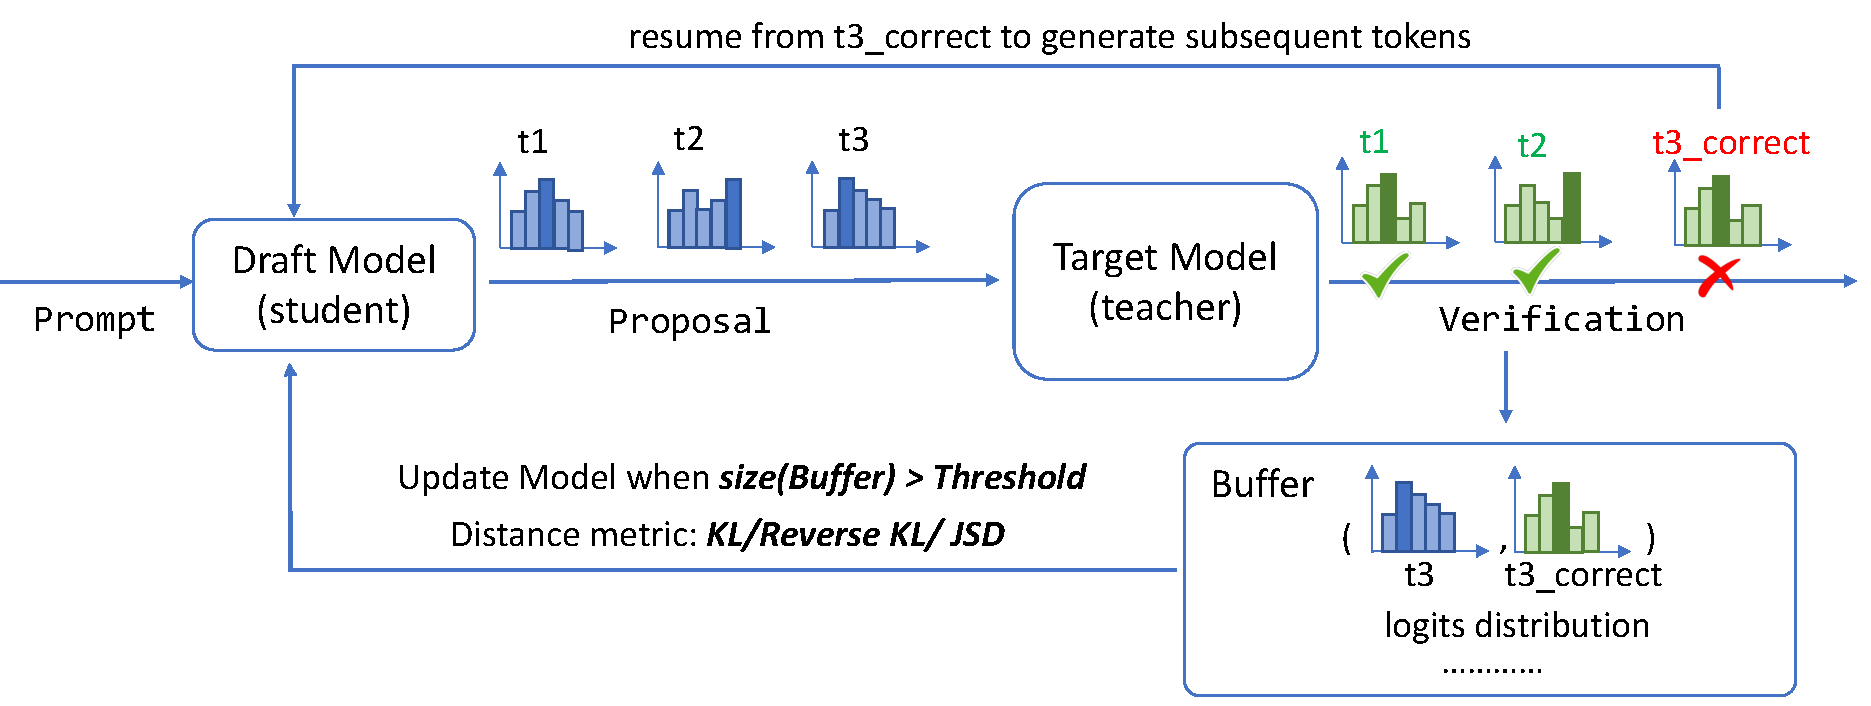
\includegraphics[width=0.8\linewidth]{figures/arch.pdf}
    \caption{Online speculative decoding overview. For each prompt, the draft model suggests multiple tokens in a single step. The target model then verifies these tokens, accepting some and rejecting others. If the student proposes incorrect tokens, both the draft and target distributions are stored in a buffer. Once the buffer exceeds a specified threshold, the draft model is updated by calculating the loss between the draft and target distributions using various distance metrics.}
\end{figure}

In summary, this paper makes the following contributions:
\begin{itemize}[leftmargin=*]
    \item We introduce online speculative decoding to reduce LLM serving latency by adapting (multiple) draft models on the fly using query data and knowledge distillation.
    \item We explore various GKD methods for constructing draft models and identify the most effective variants, suggesting them as superior alternatives to existing finetuning methods in offline settings.
    \item Our method demonstrates a significant improvement in token acceptance rate by 10-65\% on diverse datasets, translating to 1.2-3.1$\times$ reduction in latency theoretically, with a negligible additional cost. It surpasses existing methods which construct static draft models using fine-tuning or distillation on offline datasets, and matches the hypothetical accuracy achieved if all query data were available a priori.
\end{itemize}






